\section{Drive Box Assembly}

The drive box is an aluminum structure build to house the external belt drive system. It consists of four separate aluminum plates bolted together around the perimeter for modular assembly. Three of the plates are structural, while the fourth frontmost plate serves only a sealing purpose. There are five separate bearing housings protruding from the drive box and bolted to the structural plates: three in the front (the wheel shaft passes through two of them), and two in the back. The pivot is bolted through the back plate. The drive box is shown in Figures~\ref{fig:box_bld} and~\ref{fig:box_in}. Buna-N o-rings are installed between each separate component of the drive box to ensure proper sealing.

\begin{figure}[htbp]
\centering
\begin{minipage}{0.45\linewidth} \centering
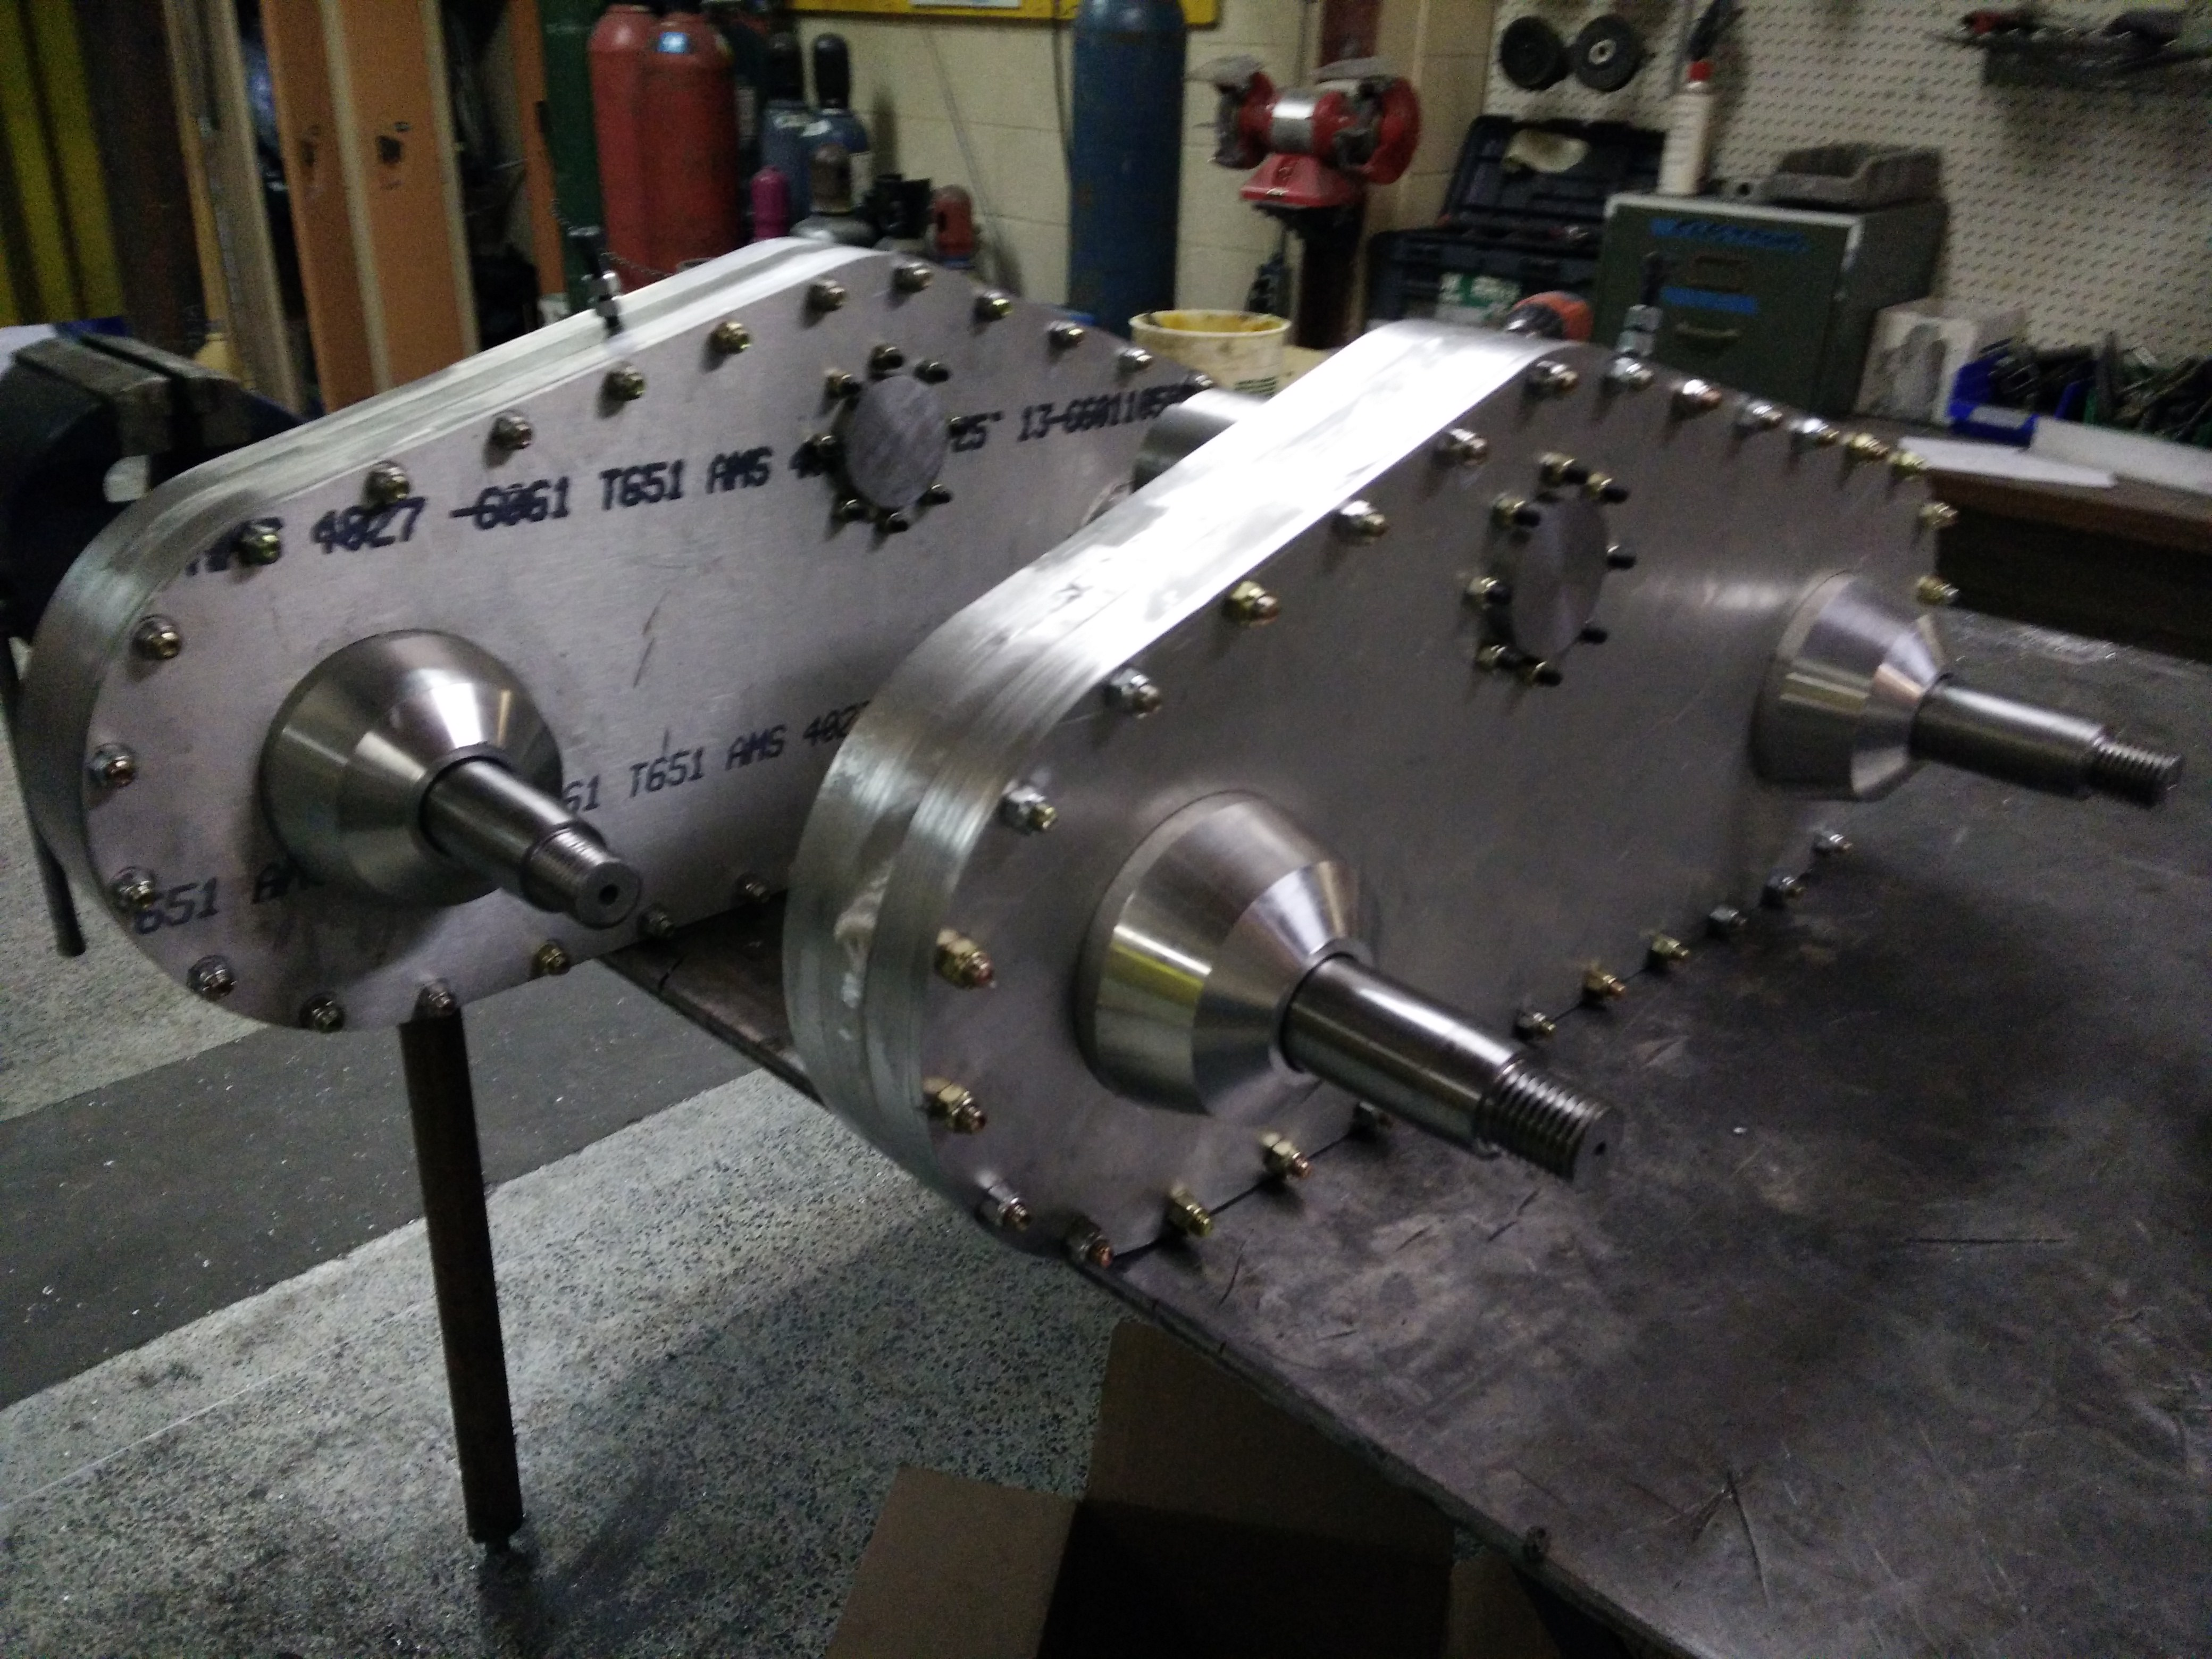
\includegraphics[height=0.22\textheight]{images/drive_box_assembly_NEW_bld}
\captionof{figure}[Completed Drive Boxes]{Two completed drive boxes before being mounted on the robot. One is the mirror image of the other.}
\label{fig:box_bld}
\end{minipage}
\hfill
\begin{minipage}{0.45\linewidth}
\centering
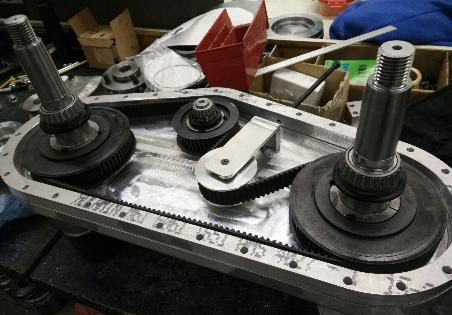
\includegraphics[height=0.22\textheight]{images/drive_box_open_bld}
\captionof{figure}[Interior of the Drive Boxes]{The drive box houses two wheel shaft assemblies, one drive shaft assembly, the belt, and tensioner.}
\label{fig:box_in}
\end{minipage}
\end{figure}

\subsection{Design Constraints and Functional Requirements}

The main constraints imposed on the drive box design are dimensional since the drive box design is constrained by the components in houses. It houses the belts, sprockets, bearing, seals, and tensioner. These components must also be laid out as defined by the shaft design software as presented in Section~\ref{sec:wheel_shaft_assembly}. Drive box dimension constraints are summarized in Table~\ref{tab:box_dim}. The drive box must be large enough to fit all the components, with additional clearance around the belt and sprocket for installation ease.

\begin{table}[htbp]
\centering
\caption{Gearbox dimension constraints}
\begin{tabular}{| lll |}\hline
Component & Dimension & Value \\ \hline
\multirow{2}{*}{Driving sprocket} & Diameter & 5  in \\
& Width & over 1.5 in \\
\multirow{2}{*}{Wheel sprocket} & Diameter & 7.6  in \\
& Width & over 1.5 in \\ \hline
\end{tabular}
\label{tab:box_dim}
\end{table}

Component drawings for the gearbox are given in Appendix~\ref{sec:drawings}. Assembly drawings are also given with the bill of materials.

The drive boxes serve two main purposes: house the interior components from the environment and support the weight of the robot with negligible deflection. Therefore, the drive box must be adequately sealed to prevent entry of fluids and/or dust particles that can cause belts to slip. They must also be strong enough not to deflect under the weight of the robot, or under the high forces seen during skid steers. This requirement is important for the obvious reason, but it is of particular importance for a belt drive. Sprockets must not lie out of plane, as this puts point loads on the belt and decrease its life.

\subsection{Analysis and Design}

During the design phase, it was decided that the best design for the drive box consisted of a number of separate plates bolted together, with o-ring seals between each. The design was produced around the layout for the internal drive box components. The box itself was produced from 6061-T6 aluminum, as this material was in stock. Note that the proposed design was based on the analysis of 6061-T0 aluminum, which has an approximately 5 times smaller yield  strength than T6. Therefore, the change only improved the strength of the drive box, as is confirmed by the finite element analysis presented below.

Several minor changes were made after the assembly of the initial drive box. Given the tight time constraints of the project, the initial intention was to have the plates water jet cut. However, due to budget restrictions it was decided that the plates would instead be milled out in house, thus eliminating the need to have the two back-most plates separate. This alleviated some of the burden of manufacturing the plates. Also, the radii of the cutouts in the plates was increased to reduce stress concentrations.

A finite element analysis was conducted on the final design for the drive box. The results are shown in Figures~\ref{fig:box_fea1} and~\ref{fig:box_fea2} in Appendix~\ref{sec:box_fea}. Deflection was negligible, maximum stress was ${82.23\ MPa}$, well below yield strength. These results were confirmed with a deflection calculation performed in Matlab.


\subsection{Belt Tensioner}

The belt tensioner is a custom-made, static, screw adjusted tensioner. The belt sits in an aluminum pulley. Sealed roller bearings are pressed into the pulley and the assembly is pressed onto a 1045 steel shaft that fits into a aluminum bracket. A screw threaded through the drive box centre plate presses against a thin steel plate mounted on top of the bracket to tension the belt. The assembly is shown in Figure~\ref{fig:box_in} and in Figure~\ref{fig:idler}. The brackets slides along slots milled out of the drive box plates.

\begin{figure}[htbp]
\centering
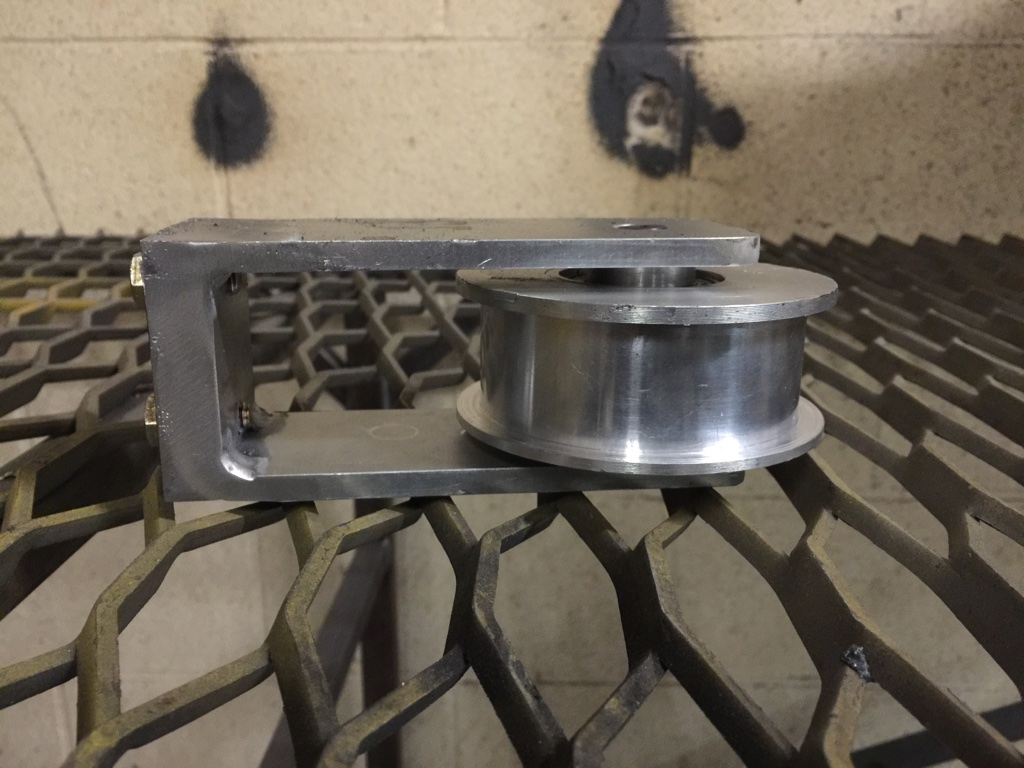
\includegraphics[height=0.3\textheight]{images/idler_assembly_bld}
\caption[Idler Assembly]{The idler assembly consists of an aluminum bracket, a thin steel plate on top, an aluminum pulley, two radial bearings and a 1045 steel shaft.}
\label{fig:idler}
\end{figure}

\subsubsection{Design and Analysis}

The tensioner must withstand the loads applied by the tensioned belt. Therefore, an FEA analysis was conducted on the assembly. For the analysis, the top of the bracket was held fixed, and a load of 5600 N was applied to the shaft in a vertical upward direction. The results showed that the maximum displacement experienced by the tensioner was ${3.162*10^{-2}}$ mm and the maximum stress in 53.76 MPa, well below the yield strength of 1045 steel. These results were confirmed with deflection calculations in Matlab, yielding a deflection of ${4.1913*10^{-2}}$ mm. The results are shown in Figure~\ref{fig:idler_fea1} and~\ref{fig:idler_fea2} in Appendix~\ref{sec:idler_fea}.


